\documentclass[a4paper, 12pt]{scrartcl}
\usepackage{amsfonts}
\usepackage[a4paper]{geometry}
\usepackage{alltt}
\usepackage{lmodern}
\usepackage{amssymb}
\usepackage{mathtools}
\usepackage{amsmath}
\usepackage{enumerate}
\usepackage{float}
\usepackage{graphicx}
\usepackage{array}
\usepackage{listings}
\usepackage{fullpage}
\usepackage[parfill]{parskip}
\usepackage[utf8]{inputenc}
\usepackage[english]{babel}

\graphicspath{ {images/} }

\title{Space Rave Documentation}
\subtitle{Interactive Visual Computing WiSe 14/15}
\author{Arne Beer, MN 6489196\\
Rafael Epplee, MN 6269560\\
Sven-Hendrik Haase, MN 6341873}

\begin{document}
\maketitle \section{Introduction}

    For our IVC project ``Space Rave'', we set out to explore the emotional impact of a music video
    that is synchronized to the contemporary electronic dance music song ``Strobe'' by Deadmau5. We
    chose this song due to its regular profile and agreeable electronic character.  The video
    consists of three distinct scenes while the visuals are set to up to represent an abstract
    spacescape throughout the scenes. The visuals consist of procedurally generated stars which
    pulse rythmically and swiftly with every kick, a procedural, fluctuating background nebula and
    a tastefully hand-modelled spaceship.

    From a technical standpoint, we used POV-Ray to generated the images and Audacity to analyze
    the music to find beats and chords. The timings were particuarly hard to get right.

    It should be noted that while we do not own the rights to the song we used, we believe that we
    are using this song in good faith in our transformative work under Fair Use.

    \section{Extracting rythm information from the sound file}

    Since POV-Ray does come with any kind of Fourier transformation, we had to analyze the song by
    hand with Audacity. While this worked fairly well, we had to be very careful about the
    sub-second timings which are easy to offset by a few milliseconds which ruins the whole
    experience.

    \begin{figure}[H]
        \centering
        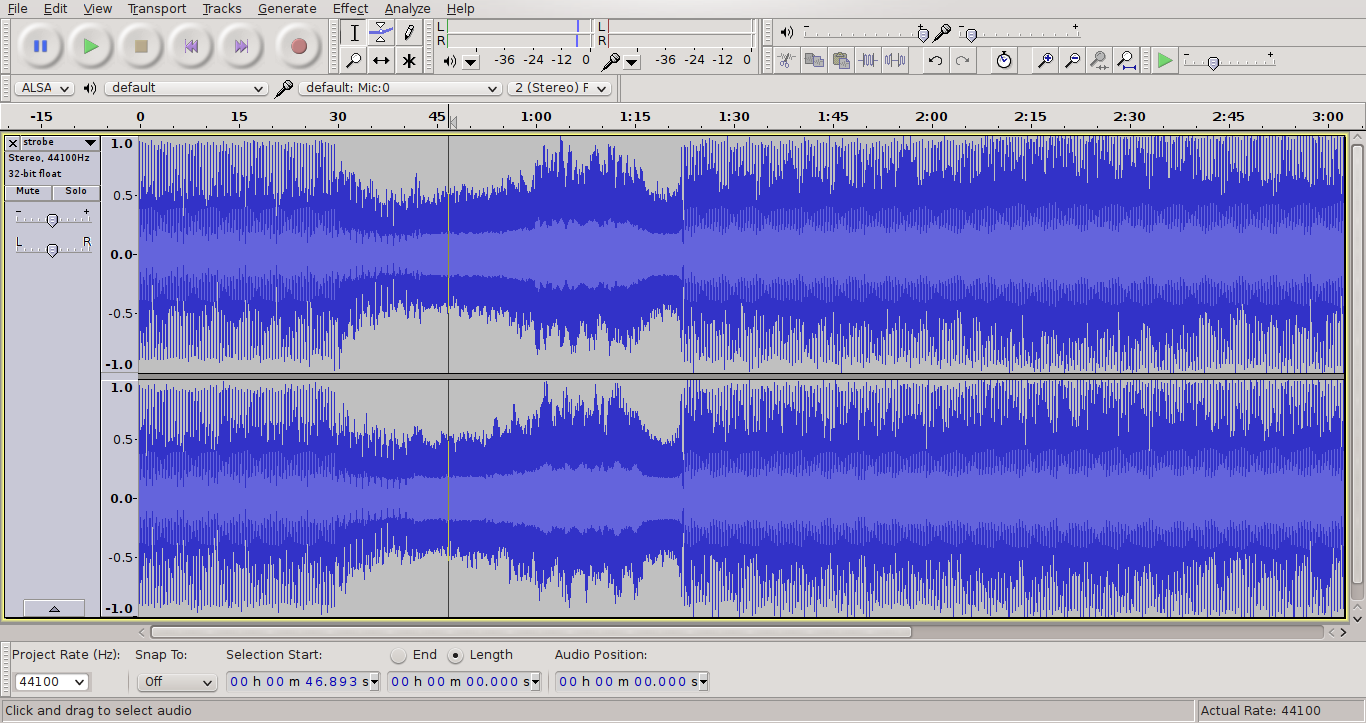
\includegraphics[scale=0.4]{audacity_main}
        \caption{Audacity main view of the track}
    \end{figure}

    \begin{figure}[H]
        \centering
        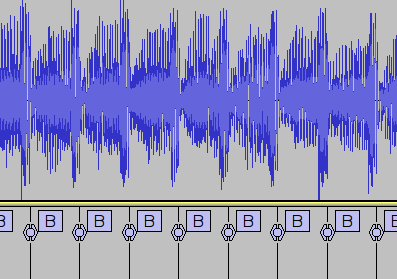
\includegraphics{audacity_beat}
        \caption{Beat analysis using Audacity's beat finder}
    \end{figure}

    \begin{figure}[H]
        \centering
        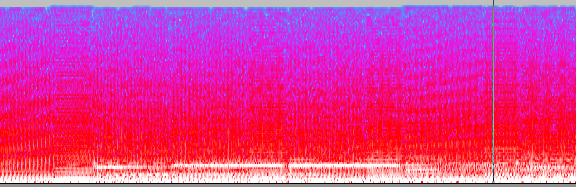
\includegraphics{audacity_spectrum}
        \caption{Spectrum view}
    \end{figure}

    \section{Modeling the Spaceship}
    We didn't use any modeling tool for making the spaceship. Instead, we opted for a blocky, ``minecrafty'' style with almost no details. We used unions to combine mostly boxes and prisms into quite a basic shape. Even the most complex part, the claws, are built with boxes and prisms.

    The size of the ship itself and various parts is easily customizable through local values declared at the top of \texttt{ship.inc}.

    Most parts of the ship are actually mirror-symmetric, like the base body, the claws and the window in the front. To minimize effort, we just modeled those parts in half and then mirrored them using duplication and scaling.

    The only non-symmetric parts of the ship are the engines at the rear end. They are each modeled on their own, each having a distinctive color.

    \section{Timing animations according to the song}

    \section{Background Generation}
    To create a starfield and nebula we used a comination of 2 spheres and a sky\_sphere. \\ 
    The sky\_sphere got a pigment that gets a perlin noise pigment map, which consists of three different colormaps. As a result we generate the procedural starfield. \\
    In order to generate a nebula we create spheres and define the interior of those. There are two different spheres with different interior medias. \\
    The first nebula is generated by creating a hollow, transparent sphere and filling it with an interior, which is defined by a media that got 2 different densities. A density is used to vary the density of particles inside a media.
    By adding two densities we get the intersection of both densities. The first density is defined by a rampwave on a colormap, to get a nice transition for the colors. We decided to spice this up by translating, warping everything and translating it back. As a result we get a nice nebula effect. \\
    The second density simply defined by a rampwave on a colormap and different density values inside the color map.

    The other sphere is quite similar to the first one, except that it got other colors, a single density and we actually vary the turbulence of density to the beat to create a wobbly effect on the nebula. 
    We use some other values like octaves, frequency and labmda to create diffent nebula look.

    \section{Ship movement}
    The movement of the last ship in the last scene has been achieved by using a spline. We use a natural\_spline to create a smoother trajectory. The spline is applied by using Trans\_Spline with pretty high values for foresight and banking, because the ship actually moves at -60*y per second.

    \section{Summary}

\end{document}
